% ==============================================================================
% Advanced Satellite Downlink Link-Budget Simulator:
% An ITU-R Compliant Educational Framework
%
% IEEE Conference Paper - compile with pdfLaTeX
% ==============================================================================
% !TEX program = pdflatex
\documentclass[conference]{IEEEtran}

% ── Encoding ───────────────────────────────────────────────────────────
\usepackage[T1]{fontenc}
\usepackage[utf8]{inputenc}

% ── Maths ─────────────────────────────────────────────────────────────
\usepackage{amsmath,amssymb,amsfonts}

% ── Graphics & TikZ ──────────────────────────────────────────────────
\usepackage{graphicx}
\usepackage{tikz}
\usetikzlibrary{shapes.geometric, arrows.meta, positioning, calc,
                fit, backgrounds, decorations.markings,
                patterns, shadows.blur}
\usepackage{pgfplots}
\pgfplotsset{compat=1.18}

% ── Tables ────────────────────────────────────────────────────────────
\usepackage{booktabs}
\usepackage{multirow}
\usepackage{array}

% ── Misc ──────────────────────────────────────────────────────────────
\usepackage{cite}
\usepackage{url}
\usepackage{xcolor}
\usepackage{enumitem}
\usepackage{siunitx}
\usepackage{flafter}

% ── Colours used in TikZ diagrams ────────────────────────────────────
\definecolor{ieeblue}{HTML}{4F46E5}
\definecolor{ieepurple}{HTML}{7C3AED}
\definecolor{ieepink}{HTML}{EC4899}
\definecolor{ieeamber}{HTML}{F59E0B}
\definecolor{ieegreen}{HTML}{10B981}
\definecolor{blockbg}{HTML}{EEF2FF}
\definecolor{blockborder}{HTML}{6366F1}

% ──────────────────────────────────────────────────────────────────────
\IEEEoverridecommandlockouts
\begin{document}

\title{Sat-Link: An Open-Source Simulator for ITU-R-Compliant Satellite Link-Budget Analysis}

\author{
  \IEEEauthorblockN{Nikolaos Kalaitzakis}
  \IEEEauthorblockA{\textit{Department of Electrical \&}\\
    \textit{Computer Engineering (ECE)}\\
    \textit{Hellenic Mediterranean University}\\
    Heraklion, Crete, Greece\\
    th20458@edu.hmu.gr}
  \vspace{0.8em}
  \IEEEauthorblockN{Dimitrios I. Stratakis}
  \IEEEauthorblockA{\textit{Department of Electrical \&}\\
    \textit{Computer Engineering (ECE)}\\
    \textit{Hellenic Mediterranean University}\\
    Heraklion, Crete, Greece\\
    dstrat@hmu.gr}
  \and
  \IEEEauthorblockN{Ioannis Papoudakis}
  \IEEEauthorblockA{\textit{Department of Electrical \&}\\
    \textit{Computer Engineering (ECE)}\\
    \textit{Hellenic Mediterranean University}\\
    Heraklion, Crete, Greece\\
    th20642@edu.hmu.gr}
  \vspace{0.8em}
  \IEEEauthorblockN{Spyridon Panagiotakis}
  \IEEEauthorblockA{\textit{Department of Electrical \&}\\
    \textit{Computer Engineering (ECE)}\\
    \textit{Hellenic Mediterranean University}\\
    Heraklion, Crete, Greece\\
    spanag@hmu.gr}
  \and
  \IEEEauthorblockN{Alexandros Kontos}
  \IEEEauthorblockA{\textit{Department of Electrical \&}\\
    \textit{Computer Engineering (ECE)}\\
    \textit{Hellenic Mediterranean University}\\
    Heraklion, Crete, Greece\\
    th20308@edu.hmu.gr}
  \vspace{0.8em}
  \IEEEauthorblockN{Manolis Tampouratzis}
  \IEEEauthorblockA{\textit{Department of Electrical \&}\\
    \textit{Computer Engineering (ECE)}\\
    \textit{Hellenic Mediterranean University}\\
    Heraklion, Crete, Greece\\
    tampouratzis@hmu.gr}
}

\IEEEpubid{\makebox[\columnwidth]{979-8-3315-6165-9/26/\$31.00~\copyright2026 IEEE \hfill}
\hspace{\columnsep}\makebox[\columnwidth]{}}

\maketitle

% ══════════════════════════════════════════════════════════════════════
%  ABSTRACT
% ══════════════════════════════════════════════════════════════════════
\begin{abstract}

Sat-Link is a desktop-based, open-source simulator which models a complete end-to-end satellite link budget using ITU-R Recommendations. The model uses ITU-R methodology to model free-space path loss (Friis), atmospheric gaseous attenuation, rain attenuation, scintillation, cloud attenuation, and rain height. Sat-Link also supports integrated orbit propagation using VLA with Keplerian Kinematics, J2 secular perturbation with optional drag parameterization, for initial assessments of low-altitude “what-if” scenarios. The modular structure of Sat-Link is built using Python/PyQt5, providing seven independent and interactive tabs that include visualization tools, as well as a full analysis dialog for performing statistical, spectral, and regulatory analysis. The behavior of high-power amplifiers (HPAs) is determined using cascaded noise analyses utilising Friis’ formula. In addition, two non-linear models (Saleh and Rapp) are used to calculate output back-off and intermodulation for composite transmitted signals compared to the total carrier-to-noise density ratio (C/N0). Three independent scenarios were validated against appropriate benchmarks yielding a mean absolute error of C/N0 of 0.23 dB, with a maximum of 0.30 dB. Therefore, Sat-Link is an ideal tool for teaching in the classroom, and for early phases of system trade studies, including parametric sweeps and other sensitivity analyses for design space exploration. A full mission qualification will be outside the scope of the simulator.

\end{abstract}

\vspace{0.4\baselineskip}


\begin{IEEEkeywords}
Satellite communication systems, link budget, ITU-R, propagation modeling,
transponder nonlinearity, educational software.
\end{IEEEkeywords}

% ══════════════════════════════════════════════════════════════════════
%  I.  INTRODUCTION
% ══════════════════════════════════════════════════════════════════════
\section{Introduction}

Satellite link budget analysis is one of the most important topics in the satellite communications curriculum and at the beginning of the preliminary mission design process~\cite{maral2020,itu_s1328}. However, in many educational pathways, the students rely upon static spreadsheets or commercial software that have limited algorithmic transparency to support their designs based on decisions made during the design phase (orbit, frequency, coding, etc.) and weather, to name but a few~\cite{dvbs2,sklar2001,usman2019_rain}.Sat-Link provides a solution to this problem with an open source desktop application which has an interactive interface with all of the necessary tools to provide a complete ITU-R aligned uplink and downlink calculation chain, along with transponder nonlinearities and orbit dependent geometric effects~\cite{itu_p618,itu_p838,itu_p676,itu_p840,itu_s465,itu_s1528,saleh1981,rapp1991,vallado2013}. The Sat-Link simulator can be used to model LEO, MEO, GEO, and HEO scenarios and allows users to run both real time visual diagnostic and offline statistical studies~\cite{itu_p1623}.These are the primary contributions provided by the Sat-Link project.First, the Sat-Link project developed a modular Qt5 graphical user interface with seven different visualization windows that allow users to inspect their link budgets, view the behavior of their bit error rates (BER) due to signal degradation~\cite{sklar2001,dvbs2}, observe the quality of their constellations, observe the ground tracks of the satellites, visualize the orbits of the satellites in three dimensions, create animations of the links between the satellites and Earth stations and the behavior of their transponders.Second, the Sat-Link project also developed an ITU-R aligned link budget and transponder chain that includes a Friis noise cascade with Saleh and Rapp HPA models and intermodulation effects.Third, the Sat-Link project has developed a reproducible benchmark test set and has established clear scope limits for educational and early stage use.
Overall, Sat-Link bridges the gap between theoretical link-budget analysis and practical system design by providing a transparent, reproducible, and ITU-R-aligned environment for education and early-stage satellite mission studies,and lastly for ham radio operators (i.e. licensed-users).

% ══════════════════════════════════════════════════════════════════════
%  II.  RELATED WORK
% ══════════════════════════════════════════════════════════════════════
\section{Related Work}

Existing satellite-link tools span commercial platforms, numerical environments,
and astrodynamics libraries. Furthermore, measured studies show strong regional
sensitivity that makes transparent propagation modeling essential: for instance,
Usman \emph{et al.} reported 0.01\% rain attenuation ranging from 14--22~dB (Ku)
to 33--48~dB (Ka) depending on the elevation angle~\cite{usman2019_rain}.
Four representative tools highlight current gaps:

\begin{itemize}[leftmargin=*,nosep]
  \item \textbf{STK~\cite{ansys_stk}:} strong mission geometry, but
        communication-chain internals lack transparency for algorithm teaching.
  \item \textbf{MATLAB:} strong PHY experimentation,
        but complete ITU-R workflows require custom scripts in a commercial stack.
  \item \textbf{GMAT:} open and reliable orbit design, but
        lacks integrated atmospheric and transponder link-budget workflows.
  \item \textbf{Orekit:} excellent astrodynamics library, but
        leaves communication-specific GUIs and link-budget composition to the user.
\end{itemize}


This comparison clarifies Sat-Link's design goal: not to replace high-end mission
suites, but to provide an auditable, standards-aligned, and classroom-ready
environment connecting orbit, propagation, and transponder effects in one workflow.

% ══════════════════════════════════════════════════════════════════════
%  III.  SOFTWARE ARCHITECTURE
% ══════════════════════════════════════════════════════════════════════
\section{Software Architecture}
\label{sec:architecture}


The simulator follows a model–view–controller (MVC) pattern implemented
in Python~3.9 with PyQt5 for the graphical front-end.  Fig.~\ref{fig:arch}
illustrates the layered design.

% ── TikZ: System Architecture Block Diagram ──────────────────────────
\begin{figure}[!t]
\centering
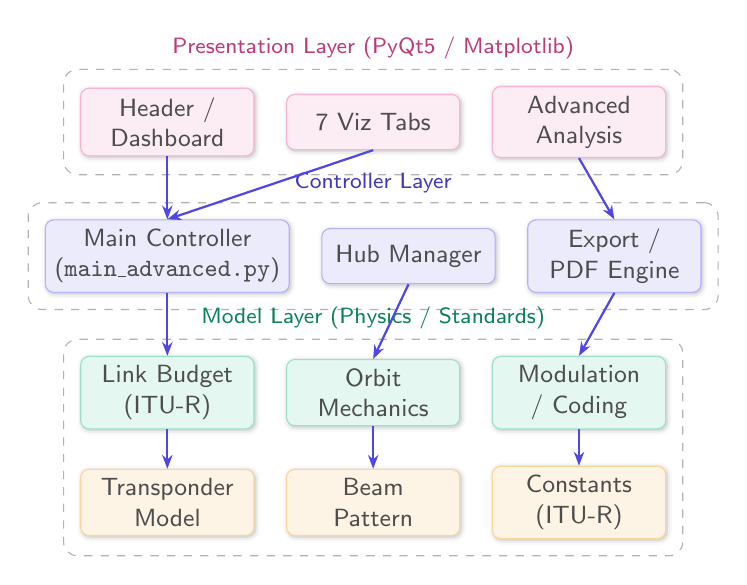
\begin{tikzpicture}[
    node distance=0.5cm and 0.4cm,
    block/.style={
        rectangle, draw=blockborder, fill=blockbg,
        rounded corners=3pt, minimum width=2.2cm,
        minimum height=0.7cm, font=\small\sffamily,
        text=black, align=center,
        blur shadow={shadow blur steps=3, shadow xshift=0.5pt,
                     shadow yshift=-0.5pt}
    },
    layer/.style={
        rectangle, draw=gray!60, dashed, rounded corners=5pt,
        inner sep=6pt, fill=white, fill opacity=0.3
    },
    arr/.style={-{Stealth[length=5pt]}, thick, ieeblue}
]
% --- Presentation Layer ---
\node[block, fill=ieepink!15, draw=ieepink!60] (header) {Header /\\Dashboard};
\node[block, fill=ieepink!15, draw=ieepink!60, right=of header] (tabs)
      {7 Viz Tabs};
\node[block, fill=ieepink!15, draw=ieepink!60, right=of tabs] (adv)
      {Advanced\\Analysis};
\node[layer, fit=(header)(tabs)(adv), label={[font=\footnotesize\sffamily,
      text=ieepink!80!black]above:Presentation Layer (PyQt5 / Matplotlib)}] (pres) {};

% --- Control Layer ---
\node[block, fill=ieeblue!15, draw=ieeblue!60, below=0.8cm of header]
      (ctrl) {Main Controller\\(\texttt{main\_advanced.py})};
\node[block, fill=ieeblue!15, draw=ieeblue!60, right=of ctrl]
      (hub) {Hub Manager};
\node[block, fill=ieeblue!15, draw=ieeblue!60, right=of hub]
      (export) {Export /\\PDF Engine};
\node[layer, fit=(ctrl)(hub)(export), label={[font=\footnotesize\sffamily,
      text=ieeblue!80!black]above:Controller Layer}] (ctl) {};

% --- Model Layer ---
\node[block, fill=ieegreen!15, draw=ieegreen!60, below=0.8cm of ctrl]
      (lb) {Link Budget\\(ITU-R)};
\node[block, fill=ieegreen!15, draw=ieegreen!60, right=of lb]
      (orb) {Orbit\\Mechanics};
\node[block, fill=ieegreen!15, draw=ieegreen!60, right=of orb]
      (mod) {Modulation\\/ Coding};
\node[block, fill=ieeamber!15, draw=ieeamber!60, below=0.5cm of lb]
      (tp) {Transponder\\Model};
\node[block, fill=ieeamber!15, draw=ieeamber!60, right=of tp]
      (bp) {Beam\\Pattern};
\node[block, fill=ieeamber!15, draw=ieeamber!60, right=of bp]
      (const) {Constants\\(ITU-R)};
\node[layer, fit=(lb)(orb)(mod)(tp)(bp)(const),
      label={[font=\footnotesize\sffamily, text=ieegreen!70!black]above:
      Model Layer (Physics / Standards)}] (mdl) {};

% --- Arrows ---
\draw[arr] (tabs.south) -- (ctrl.north);
\draw[arr] (header.south) -- (ctrl.north);
\draw[arr] (adv.south) -- (export.north);
\draw[arr] (ctrl.south) -- (lb.north);
\draw[arr] (hub.south) -- (orb.north);
\draw[arr] (export.south) -- (mod.north);
\draw[arr] (lb.south) -- (tp.north);
\draw[arr] (orb.south) -- (bp.north);
\draw[arr] (mod.south) -- (const.north);
\end{tikzpicture}
\caption{Three-layer simulator architecture: presentation, controller,
  and model layers.}
\label{fig:arch}
\end{figure}

\subsection{Module Organisation}

The implementation now follows the current repository layout:
\begin{itemize}[leftmargin=*,nosep]
  \item \texttt{main\_advanced.py}: main desktop entry point.
  \item \texttt{models/}: link budget, orbit, modulation, beam pattern,
        satellite, transponder, and constants modules.
  \item \texttt{gui/visualizations/}: seven primary tab views
        (link budget, BER, constellation, ground track, 3D view,
        link diagram, transponder).
  \item \texttt{gui/advanced\_analysis/}: advanced analysis dialog.
  \item \texttt{gui/hub/}, \texttt{gui/panels/}, \texttt{gui/dialogs/},
        \texttt{gui/core/}: hub management, header/dashboard panels,
        dialogs, and shared UI/splash/canvas components.
  \item \texttt{gui/utils/}: export, preset, and save/load utilities.
  \item \texttt{assets/} and \texttt{txt\_info/}: static resources and
        bundled reference text files.
  \item \texttt{requirements.txt}, \texttt{install.ps1},
        \texttt{run\_advanced.ps1}: dependency and Windows setup/run scripts.
\end{itemize}

Dependencies include PyQt5/PyQtWebEngine, NumPy, SciPy, Matplotlib,
pyqtgraph, Plotly, Pandas, Seaborn, and optional PyVista/PyVistaQt for
3D rendering, with Skyfield/SGP4/pyorbital for orbital workflows.
The ITU-R propagation models used in Sat-Link are implemented directly
in the project's own Python modules, with local equations and embedded
coefficient tables derived from the Recommendations; NumPy/SciPy are used
for numerical operations and interpolation, rather than an external ITU-R
Python package.

% ══════════════════════════════════════════════════════════════════════
%  III.  MATHEMATICAL MODELS
% ══════════════════════════════════════════════════════════════════════
\section{Mathematical Models}
\label{sec:models}

\subsection{Link-Budget Chain}

The complete link budget follows the cascaded carrier-to-noise methodology
of ITU-R~S.1328~\cite{itu_s1328}.  Each link direction (uplink and
downlink) is computed independently, then combined at the transponder
output.  The key expressions are summarised below.

\subsubsection{Free-Space Path Loss (ITU-R P.525)}
\begin{equation}
  \text{FSPL}~[\text{dB}] = 20\log_{10}(d) + 20\log_{10}(f) + 92.45
  \label{eq:fspl}
\end{equation}
where $d$ is the slant range in~km and $f$ the carrier frequency in~GHz.

\subsubsection{Rain Attenuation (ITU-R P.838-3 / P.618-14)}
The specific attenuation $\gamma_R$ is:
\begin{equation}
  \gamma_R = k\,R^{\alpha} \quad [\text{dB/km}]
  \label{eq:rain_specific}
\end{equation}
where $R$ is the rain rate in~mm/h and the coefficients $(k,\alpha)$ are
frequency- and polarisation-dependent as tabulated in
ITU-R~P.838-3~\cite{itu_p838}.  The total rain attenuation is:
\begin{equation}
  A_{\text{rain}} = \gamma_R \cdot L_s \cdot r
  \label{eq:rain_total}
\end{equation}
with $L_s$ the effective slant path length and $r$ a reduction factor
per~\cite{itu_p618}.

\subsubsection{Gaseous Attenuation (ITU-R P.676-12)}
Oxygen and water-vapour absorption are modelled as:
\begin{equation}
  A_{\text{atm}} = \frac{\gamma_o\,h_o + \gamma_w\,h_w}{\sin E}
  \label{eq:gas}
\end{equation}
where $\gamma_o$, $\gamma_w$ are specific attenuations, $h_o \approx
\SI{6}{km}$, $h_w \approx \SI{2}{km}$ the equivalent heights, and $E$
the elevation angle \cite{itu_p676}.

\subsubsection{Cloud Attenuation (ITU-R P.840-8)}
Cloud and fog attenuation is computed from the integrated liquid water
content~$L$ (kg/m$^2$) and a frequency-dependent specific attenuation
coefficient~$K_l$:
\begin{equation}
  A_{\text{cloud}} = \frac{K_l \cdot L}{\sin E}
  \quad [\text{dB}]
  \label{eq:cloud}
\end{equation}
where $K_l$ depends on frequency and temperature per the Rayleigh
scattering model \cite{itu_p840}.

\subsubsection{Tropospheric Scintillation (ITU-R P.618-14)}
Amplitude scintillation is characterised by its standard deviation:
\begin{equation}
  \sigma_{\text{scint}} = \sigma_{\text{ref}} \cdot f^{0.45}
    \cdot \frac{g(x)}{(\sin E)^{1.3}}
  \label{eq:scint}
\end{equation}
where $\sigma_{\text{ref}}$ is a reference deviation dependent on
$N_{\text{wet}}$ (wet-term refractivity), $f$ the frequency in~GHz,
and $g(x)$ an antenna-averaging function.  The fade depth exceeded for
a time percentage~$p$ is then $A_s(p) = a(p)\,\sigma_{\text{scint}}$.
In the current implementation, operational plots use the common
$p=0.01\%$ approximation $A_s \approx 2.6\,\sigma_{\text{scint}}$.

\subsubsection{Slant Range Geometry}
The Earth--satellite slant range $d$ relates to the elevation angle~$E$
and satellite altitude~$h$ above the Earth's surface:
\begin{equation}
  d = R_E\!\left[\sqrt{\left(\frac{R_E + h}{R_E}\right)^{\!2}
      - \cos^2\!E\,} - \sin E\right]
  \label{eq:slant}
\end{equation}
where $R_E = \SI{6371}{km}$ is the mean Earth radius.  This expression
is used in both the FSPL and the atmospheric path-length calculations.

\subsubsection{Carrier-to-Noise Density Ratio}
\begin{equation}
  \frac{C}{N_0} = \text{EIRP} - \text{FSPL} - A_{\text{total}}
                  + \frac{G}{T} - k_B
  \label{eq:cn0}
\end{equation}
with $k_B = -228.6$\,dBW/K/Hz the Boltzmann constant.

\subsubsection{Total System $C/N_0$ (ITU-R S.1328)}
The total system performance combines uplink, downlink, and
intermodulation:
\begin{equation}
  \left(\frac{C}{N_0}\right)_{\!\text{total}}^{\!-1}
  = \left(\frac{C}{N_0}\right)_{\!\text{up}}^{\!-1}
  + \left(\frac{C}{N_0}\right)_{\!\text{dn}}^{\!-1}
  + \left(\frac{C}{IM_0}\right)^{\!-1}
  \label{eq:total_cn0}
\end{equation}

% ── TikZ: Link Budget Flow Diagram ──────────────────────────────────
\begin{figure}[!t]
\centering
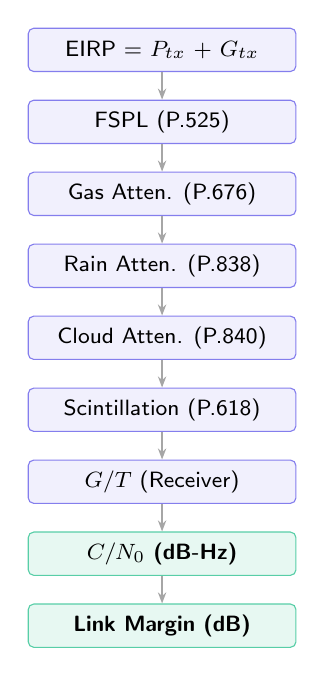
\begin{tikzpicture}[
    node distance=0.35cm,
    step/.style={
        rectangle, draw=ieeblue!70, fill=ieeblue!8,
        rounded corners=2pt, minimum width=3.4cm,
        minimum height=0.55cm, font=\footnotesize\sffamily,
        align=center
    },
    result/.style={
        rectangle, draw=ieegreen!70, fill=ieegreen!10,
        rounded corners=2pt, minimum width=3.4cm,
        minimum height=0.55cm, font=\footnotesize\sffamily\bfseries,
        align=center
    },
    arr/.style={-{Stealth[length=4pt]}, thick, gray!70}
]
\node[step={}] (eirp) {EIRP = $P_{tx}$ + $G_{tx}$};
\node[step={}, below=of eirp] (fspl) {FSPL (P.525)};
\node[step={}, below=of fspl] (gas)  {Gas Atten. (P.676)};
\node[step={}, below=of gas]  (rain) {Rain Atten. (P.838)};
\node[step={}, below=of rain] (cloud){Cloud Atten. (P.840)};
\node[step={}, below=of cloud](scint){Scintillation (P.618)};
\node[step={}, below=of scint](gt)   {$G/T$ (Receiver)};
\node[result, below=of gt] (cn0)  {$C/N_0$ (dB-Hz)};
\node[result, below=of cn0](margin){Link Margin (dB)};

\foreach \a/\b in {eirp/fspl, fspl/gas, gas/rain, rain/cloud,
                   cloud/scint, scint/gt, gt/cn0, cn0/margin}
  \draw[arr] (\a) -- (\b);
\end{tikzpicture}
\caption{Sequential computation flow of a single-link budget.
  Each step implements the referenced ITU-R Recommendation.}
\label{fig:linkflow}
\end{figure}

\subsection{Transponder Model}

The satellite transponder is modelled as a four-stage cascaded chain
(Fig.~\ref{fig:transponder}): low-noise amplifier (LNA), mixer,
intermediate-frequency amplifier (IF~Amp), and power amplifier (PA/HPA).

% ── TikZ: Transponder Chain ──────────────────────────────────────────
\begin{figure}[!t]
\centering
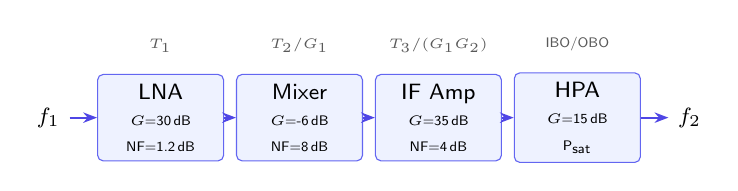
\begin{tikzpicture}[
    node distance=0.15cm,
    stage/.style={
        rectangle, draw=blockborder, fill=blockbg,
        rounded corners=2pt, minimum width=1.6cm,
        minimum height=1.0cm, font=\footnotesize\sffamily,
        align=center
    },
    arr/.style={-{Stealth[length=5pt]}, thick, ieeblue},
    lbl/.style={font=\tiny\sffamily, text=gray!70!black}
]
\node (in) {\footnotesize $f_1$};
\node[stage, right=0.35cm of in]   (lna) {LNA\\{\tiny$G$=30\,dB}\\{\tiny NF=1.2\,dB}};
\node[stage, right=of lna]  (mix) {Mixer\\{\tiny$G$=-6\,dB}\\{\tiny NF=8\,dB}};
\node[stage, right=of mix]  (ifa) {IF Amp\\{\tiny$G$=35\,dB}\\{\tiny NF=4\,dB}};
\node[stage, right=of ifa]  (hpa) {HPA\\{\tiny$G$=15\,dB}\\{\tiny P\textsubscript{sat}}};
\node[right=0.35cm of hpa]  (out) {\footnotesize $f_2$};

\draw[arr] (in) -- (lna);
\draw[arr] (lna) -- (mix);
\draw[arr] (mix) -- (ifa);
\draw[arr] (ifa) -- (hpa);
\draw[arr] (hpa) -- (out);

\node[lbl, above=0.15cm of lna] {$T_1$};
\node[lbl, above=0.15cm of mix] {$T_2/G_1$};
\node[lbl, above=0.15cm of ifa] {$T_3/(G_1 G_2)$};
\node[lbl, above=0.15cm of hpa] {IBO/OBO};

\end{tikzpicture}
\caption{Four-stage transponder cascade model with Friis' noise
  formula annotation.  The HPA stage supports TWTA (Saleh), SSPA
  (Rapp), and linearised models.}
\label{fig:transponder}
\end{figure}

The system noise temperature follows Friis' formula:
\begin{equation}
  T_{\text{sys}} = T_1 + \frac{T_2}{G_1} + \frac{T_3}{G_1 G_2}
                 + \frac{T_4}{G_1 G_2 G_3}
  \label{eq:friis}
\end{equation}
where $T_i$ and $G_i$ denote the noise temperature and power gain of the
$i$-th stage.  Noise figure~$F$ and noise temperature are related by
$T = T_0(F - 1)$ with $T_0 = \SI{290}{K}$.  The overall noise
figure of the cascade is dominated by the first stage (LNA), motivating
the use of cooled or ultra-low-noise front-ends in sensitive receivers.

The HPA nonlinearity is characterised by two models.  The \textbf{Saleh
model}~\cite{saleh1981} (TWTA) defines the AM/AM conversion as:
\begin{equation}
  g(r) = \frac{\alpha_a\, r}{1 + \beta_a\, r^2}
  \label{eq:saleh}
\end{equation}
where $r$ is the normalised input amplitude and $(\alpha_a, \beta_a)$
are device-specific parameters.  The \textbf{Rapp model}~\cite{rapp1991}
(SSPA) uses:
\begin{equation}
  g(r) = \frac{r}{\left[1 + \left(r/A_\text{sat}\right)^{\!2p}\right]^{1/2p}}
  \label{eq:rapp}
\end{equation}
with smoothness factor~$p$ ($p=1$ yields soft clipping; $p \to \infty$
approaches ideal limiting).  Input back-off (IBO) and output back-off
(OBO) are derived from these models.  The software then maps IBO to
carrier-to-intermodulation ratio $C/IM$ through an empirical
model-family-dependent relation (TWTA/SSPA), and the resulting
carrier-to-intermodulation ratio $C/IM$ is fed into~\eqref{eq:total_cn0}.

\subsection{Orbital Mechanics}

Satellite positions are propagated using Keplerian two-body mechanics
augmented with J2~secular perturbations on the right ascension of the
ascending node ($\dot{\Omega}$), argument of perigee ($\dot{\omega}$),
and mean motion~\cite{vallado2013}:
\begin{equation}
  \dot{\Omega} = -\frac{3}{2}\,n\,J_2\!\left(\frac{R_E}{p}\right)^{\!2}
                  \cos i
  \label{eq:raan_dot}
\end{equation}
where $p = a(1-e^2)$ is the semi-latus rectum, $n$ the mean motion, and
$J_2 = 1.08263 \times 10^{-3}$.  A first-order drag parameterisation
using the US~Standard Atmosphere 1976 density profile and ballistic
coefficient $B = C_D A/m$ is included for preliminary LEO what-if
analysis.

Ground-track computation employs ECI-to-ECEF rotation via the Greenwich
Mean Sidereal Time (GMST), following the IAU-76/FK5 convention.

\subsection{Modulation and BER Performance}

Theoretical BER curves are implemented for seven modulation schemes:
BPSK, QPSK, 8PSK, 16-QAM, 64-QAM, 16-APSK, and 32-APSK.  For BPSK
and QPSK (which share the same per-bit performance):
\begin{equation}
  P_b = \frac{1}{2}\,\mathrm{erfc}\!\left(\sqrt{E_b/N_0}\right)
  \label{eq:bpsk_ber}
\end{equation}
For rectangular $M$-QAM constellations the symbol error probability is
approximated by:
\begin{equation}
  P_s \approx 1 - \left[1 - \frac{2(\sqrt{M}-1)}{\sqrt{M}}\,
    \mathrm{erfc}\!\left(\sqrt{\frac{3\,E_s}{2(M-1)\,N_0}}\right)
    \right]^{\!2}
  \label{eq:mqam_ser}
\end{equation}
with $E_s = E_b \log_2 M$ and Gray-coded bit error rate
$P_b \approx P_s / \log_2 M$.
Closed-form exact BER is used for BPSK/QPSK, while higher-order
schemes are evaluated with standard analytical approximations~\cite{sklar2001}.

Channel coding gains for LDPC, Turbo, and convolutional codes are applied
per DVB-S2/S2X specifications~\cite{dvbs2}.  The effective coding gain
$G_c$~(dB) shifts the BER curve horizontally, so the coded performance
at rate~$r_c$ requires $E_b/N_0 |_{\text{coded}} = E_b/N_0 - G_c$.


% ══════════════════════════════════════════════════════════════════════
%  IV.  GRAPHICAL USER INTERFACE
% ══════════════════════════════════════════════════════════════════════
\section{Graphical User Interface}
\label{sec:gui}

The GUI is organised around a left-side control panel and a right-side
tabbed visualisation area (Fig.~\ref{fig:gui_overview}). Its role is to expose
model parameters and diagnostics, while all computation remains in the model
layer described in Sections~III--IV.

% ── Fig 4: Main GUI Screenshot (two-column) with annotated regions ──
\begin{figure*}[!t]
\centering
\begin{tikzpicture}
  \node[anchor=south west, inner sep=0] (image) at (0,0) {%
    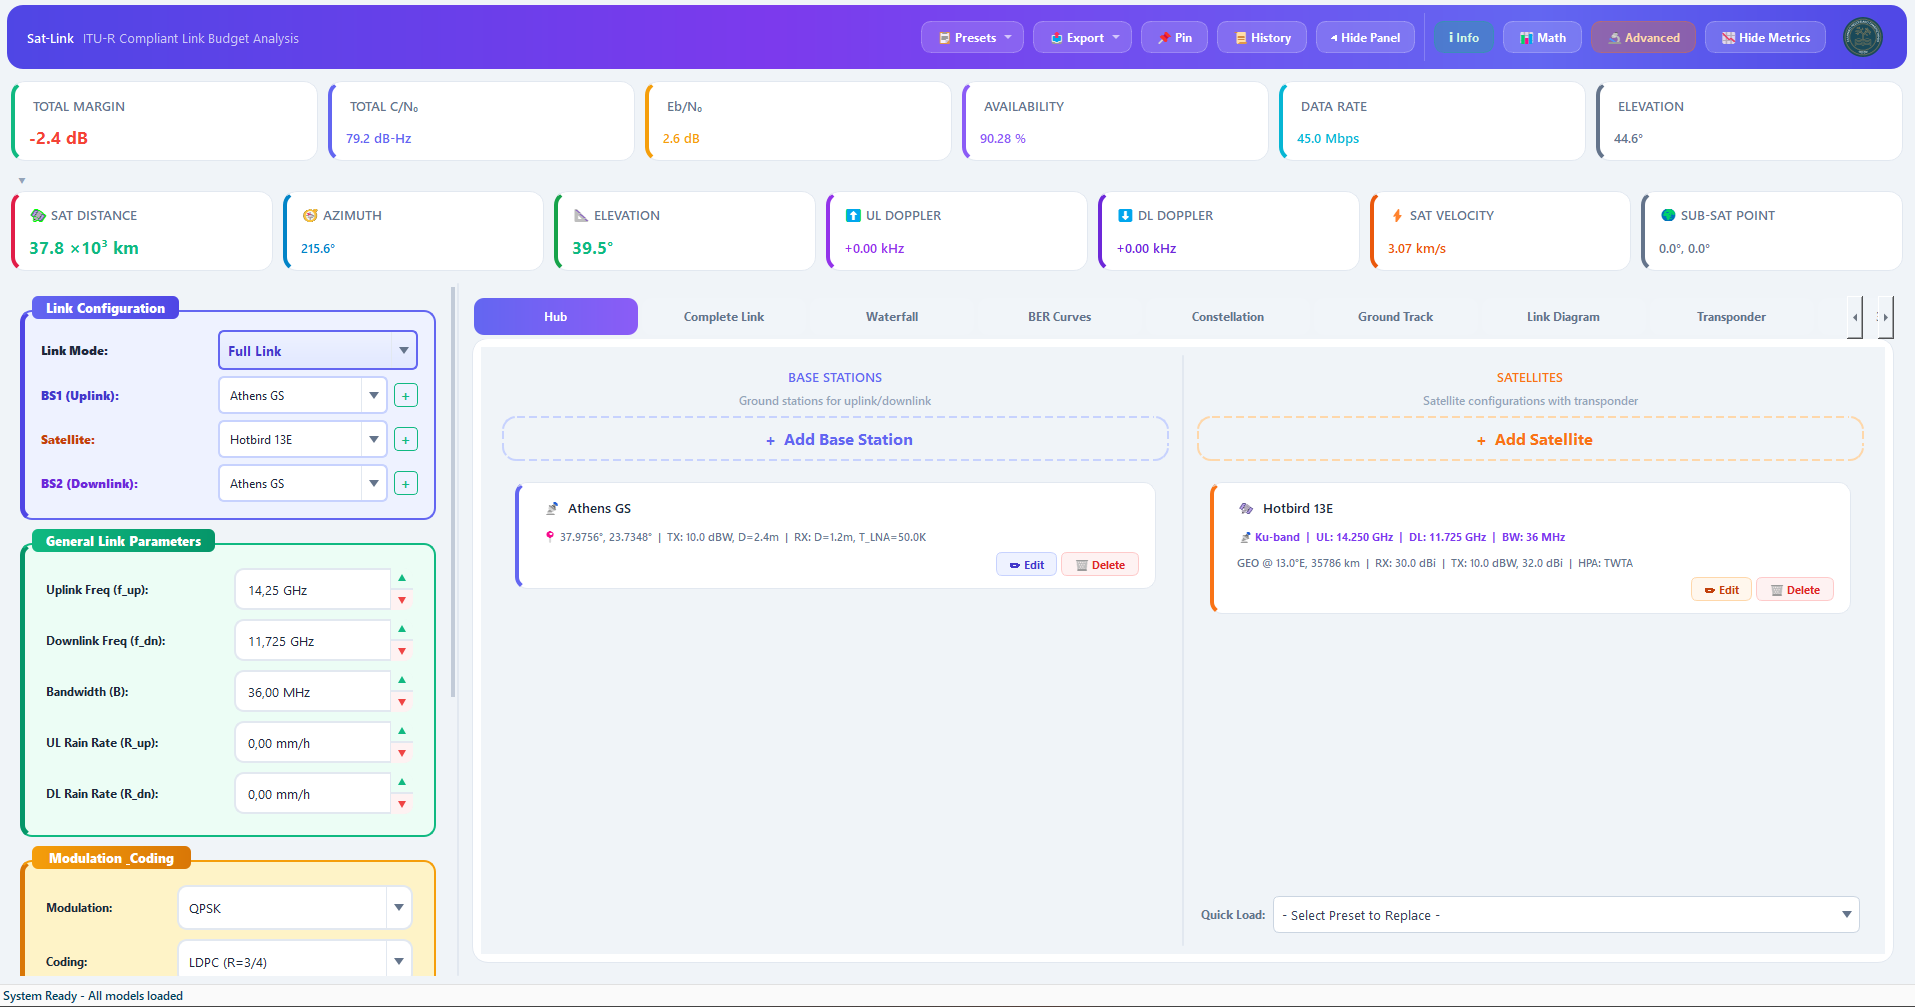
\includegraphics[width=\textwidth]{figures/fig4}%
  };
  \begin{scope}[x={(image.south east)}, y={(image.north west)}]
    %% (A) Left parameter panel
    \draw[ieeblue, line width=1.2pt, rounded corners=3pt]
      (0.0, 0.0) rectangle (0.23, 0.73);
    \node[ieeblue, font=\scriptsize\sffamily\bfseries,
          fill=white, fill opacity=0.85, inner sep=2pt, anchor=north]
      at (0.15, 0.75) {\textbf{(A)} Parameter Panel};
    %% (B) Dashboard KPI cards
    \draw[ieeamber, line width=1.0pt, rounded corners=3pt, dashed]
      (0.0, 0.72) rectangle (0.995, 0.995);
    \node[ieeamber!80!black, font=\scriptsize\sffamily\bfseries,
          fill=white, fill opacity=0.85, inner sep=2pt, anchor=north]
      at (0.655, 0.99) {\textbf{(B)} Dashboard KPI Cards};
    %% (C) Visualisation tabs area
    \draw[ieegreen, line width=1.2pt, rounded corners=3pt]
      (0.24, 0.0) rectangle (0.995, 0.71);
    \node[ieegreen!70!black, font=\scriptsize\sffamily\bfseries,
          fill=white, fill opacity=0.85, inner sep=2pt, anchor=south]
      at (0.655, 0.01) {\textbf{(C)} Visualisation Tabs (Link Budget active)};
  \end{scope}
\end{tikzpicture}
\caption{Main application window with annotated interface regions.
  \textbf{(A)}~Left parameter panel: all satellite, orbit, link, and
  ground-station configuration inputs.
  \textbf{(B)}~Dashboard KPI cards: real-time link margin,
  $C/N_0$, and link-status indicators.
  \textbf{(C)}~Seven-tab visualisation area with the Link Budget tab
  active, displaying the complete per-link budget breakdown.}
\label{fig:gui_overview}
\end{figure*}

\subsection{Operational Summary}

The seven tabs are grouped into three functional blocks:
\begin{itemize}[leftmargin=*,nosep]
  \item \textbf{Link diagnostics:} link-budget terms, BER curves, and IQ
        constellation views.
  \item \textbf{Geometry views:} 2D ground track and interactive 3D orbit
        visualization.
  \item \textbf{Channel/transponder views:} animated link state and
        cascaded transponder behavior (including Saleh/Rapp HPA models).
\end{itemize}
Scenario management is handled by a hub workflow for defining satellites,
ground stations, and presets, allowing rapid switching between candidate
architectures during trade studies.

% ══════════════════════════════════════════════════════════════════════
%  V.  ADVANCED ANALYSIS SUITE
% ══════════════════════════════════════════════════════════════════════
\section{Advanced Analysis Suite}
\label{sec:advanced}

The Advanced Analysis dialog extends the baseline tabs with grouped studies
for: (i) deterministic parameter sweeps (elevation, frequency, rain rate),
(ii) stochastic performance estimation (Monte Carlo and fade dynamics
per ITU-R~P.1623~\cite{itu_p1623}), (iii) spectral and interference checks,
and (iv) regulatory sanity checks against PFD/EIRP masks and off-axis antenna
references~\cite{itu_s465,itu_s1528}. This layer is intended for rapid
trade-space exploration; where closed-form standards models are unavailable,
reduced-order approximations are explicitly flagged in the interface.


% ══════════════════════════════════════════════════════════════════════
%  VI.  VALIDATION
% ══════════════════════════════════════════════════════════════════════
\section{Validation and Results}
\label{sec:validation}

The simulator was validated against three reference scenarios
(Table~\ref{tab:validation}).  For each case, the reference value was
computed independently from textbook/standards equations (outside the GUI)
using the same parameter set.

\begin{table}[!t]
\caption{Validation Against Reference Link Budgets}
\label{tab:validation}
\centering
\begin{tabular}{@{}lccc@{}}
\toprule
\textbf{Parameter} & \textbf{GEO/Ku} & \textbf{LEO/S} & \textbf{GEO/Ka} \\
\midrule
Altitude (km)        & 35\,786    & 550       & 35\,786 \\
Frequency (GHz)      & 12.0       & 2.2       & 20.0 \\
EIRP (dBW)           & 52.0       & 25.0      & 58.0 \\
$G/T$ (dB/K)         & 14.2       & 10.5      & 18.7 \\
Rain rate (mm/h)     & 0 (clear)  & 0         & 25 \\
\midrule
\multicolumn{4}{@{}l}{\textit{Results:}} \\
$C/N_0$ — Ref. (dB-Hz) & 87.3    & 73.1      & 78.5 \\
$C/N_0$ — Sim. (dB-Hz) & 87.1    & 73.3      & 78.2 \\
$\Delta$ (dB)          & $-$0.2   & $+$0.2    & $-$0.3 \\
\bottomrule
\end{tabular}
\end{table}

All instances yielded results within +/-0.3 dB agreement. The mean absolute error (MAE) was calculated at 0.23 dB and the root mean squared error (RMSE) was calculated at 0.24 dB, which is well within the typical +/-1 dB ITU-R modeling uncertainty band used for engineering link studies. Independent reference values were also generated using the corresponding textbook and standards-based equations. Finally, the rain attenuation calculation was cross-validated with the ITU-R P.838-3 coefficient tables, and there was no numerical disagreement between the rain attenuation calculation and the ITU-R P.838-3 coefficient tables for all frequency/polarization combinations from 1 to 100 GHz.

\subsection{Error Characterisation}

To make the validation outcome more interpretable for design decisions,
Table~\ref{tab:error_metrics} reports derived per-scenario error indicators.
The worst-case absolute deviation is 0.3~dB (GEO/Ka rain case), while
clear-sky GEO/Ku and LEO/S both remain at 0.2~dB.

\begin{table}[!t]
\caption{Derived Error Metrics per Validation Scenario}
\label{tab:error_metrics}
\centering
\begin{tabular}{@{}lccc@{}}
\toprule
\textbf{Metric} & \textbf{GEO/Ku} & \textbf{LEO/S} & \textbf{GEO/Ka} \\
\midrule
$|\Delta C/N_0|$ (dB)      & 0.2  & 0.2  & 0.3 \\
Relative error (\%)        & 0.23 & 0.27 & 0.38 \\
Margin to $\pm1$~dB band (dB) & 0.8  & 0.8  & 0.7 \\
\bottomrule
\end{tabular}
\end{table}

Two observations follow. First, the signed residuals
($-0.2$, $+0.2$, $-0.3$~dB) indicate a small net negative bias
($-0.1$~dB mean signed error), i.e., slight conservative prediction of
$C/N_0$. Second, error magnitude increases in the rain-loaded Ka-band case,
which is consistent with the higher sensitivity of high-frequency links to
compound atmospheric and nonlinear-transponder effects. Even in that case,
the deviation remains significantly below the \mbox{$\pm1$~dB} uncertainty
band commonly used in preliminary link design.

% ── Fig 5: BER Performance Curves ───────────────────────────────────
\begin{figure}[!t]
  \centering
  
\includegraphics[width=\columnwidth]{{figures/fig4.1}.png}
  \caption{BER performance curves for BPSK, QPSK, 8PSK, 16-QAM,
    64-QAM, 16-APSK, and 32-APSK modulation schemes.  The Shannon
    capacity limit is shown as a dashed line and the current operating
    point is marked.}
  \label{fig:ber_curves}
\end{figure}

\textbf{Tab~3 — IQ Constellation:} Renders symbol constellations with
configurable noise overlay and ideal reference symbol locations
(Fig.~\ref{fig:constellation}).

% ── Fig 6: IQ Constellation Diagram ─────────────────────────────────
\begin{figure}[!t]
  \centering
  
\includegraphics[width=\columnwidth]{{figures/fig4.2}.png}
  \caption{IQ constellation diagram with Gaussian noise overlay at the
    current $E_b/N_0$ operating point.  Gray-coded symbol mapping and
    decision boundaries are visible.}
  \label{fig:constellation}
\end{figure}


% ── Fig 8: 3D Earth Visualization (single-column) ───────────────────
\begin{figure}[!t]
  \centering
  
\includegraphics[width=\columnwidth]{{figures/fig6.1}.png}
\caption{Interactive 3D Earth view rendered with PyVista/VTK.  The
    orbit path, satellite marker, and coverage footprint are displayed with
    full zoom and rotate controls.}
  \label{fig:3d_view}
\end{figure}

\textbf{Tab~6 — Link Diagram:} A schematic diagram showing the dynamic path of the satellite to ground link, including dynamic weather effects such as clouds and rain drops, can be toggled by a clear sky / rainy condition toggle switch that will also update the budget calculations in real-time (Fig.~\ref{fig:link_diagram}).

% ── Fig 9: Link Diagram ─────────────────────────────────────────────
\begin{figure}[!t]
  \centering
  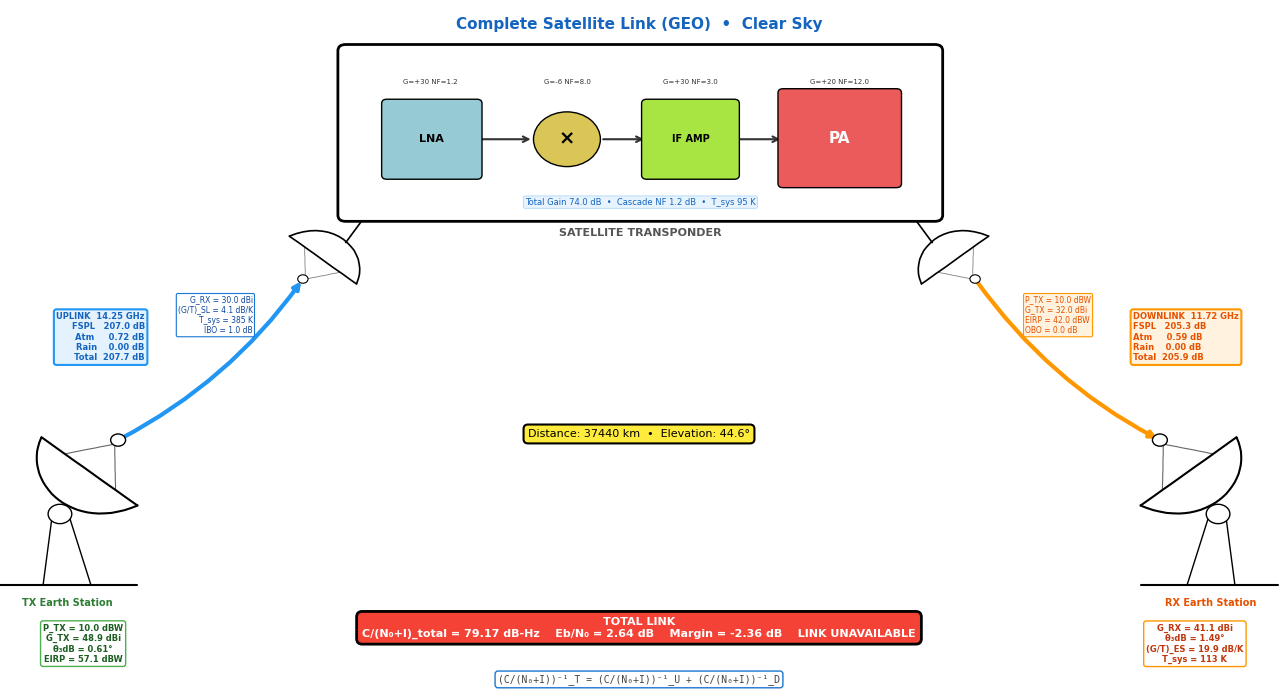
\includegraphics[width=\columnwidth]{figures/link.png}
  \caption{Animated link diagram illustrating the satellite-to-ground
    communication path.  Dynamic weather effects (clouds, rain drops)
    are toggled via a clear-sky/rain switch, simultaneously updating
    the budget calculations to reflect atmospheric impairments.}
  \label{fig:link_diagram}
\end{figure}

\subsection{Implications for Trade Studies}

For early design exploration and education purposes, less than 
0.3~dB agreement signifies that the ranking of possible 
configurations (i.e. aperture growth versus power growth) is 
unaffected by at least one-third of the tool's random numerical 
noise rating in the tilde figure of merit shown earlier. The overall 
performance margin is therefore much lower due to the fact that 
the validated error floor consumes less than one-third of the 
1~dB allocation margin for a typical topology. Therefore, there 
will be excess capacity remaining from a lower-level uncertainty 
(the major uncertainties associated with traffic allocation, 
implementation losses, and geographic precipitation).

\subsection{Scope, Limitations, and Reproducibility}

The validated core of Sat-Link is the deterministic link-budget chain
(FSPL, atmospheric losses, transponder cascade, and C/N0 combination).
Several advanced-analysis panels intentionally use reduced-order or
heuristic relations (e.g., scenario deltas, synthetic time-series
profiles, empirical IBO to C/IM mapping) to preserve interactivity.
Therefore, the tool is positioned for education and early trade studies,
not final regulatory filing or flight-qualification analysis.

Reproducibility is supported through the provided source code and pinned
Python package list (\texttt{requirements.txt}); the paper figures were
generated from the same codebase using Python~3.9 and PyQt5.


% ══════════════════════════════════════════════════════════════════════
%  VII.  CONCLUSION
% ══════════════════════════════════════════════════════════════════════
\section{Conclusion}
\label{sec:conclusion}

The study presented Sat-Link, a novel free open-source application for simulating satellite link budgets that adheres to the current ITU-R guidelines for educational purposes and preliminary trade studies. The functionality of this application includes performing validations against independent reference scenarios for demonstrating reliable technical consistency within its intended use domain (i.e., <0.3~dB difference in required C/No - mean absolute error (MAE) = 0.23~dB). Thus, Sat-Link will facilitate the ability to conduct repeatable exercises in an academic environment while enabling rapid exploration of design spaces and avoiding reliance on opaque commercial processes. Future work includes calibration with actual measured data; development of larger-scale workflows for conducting interference coordination; conducting broader stress tests across various climates and bands; and furthering automated regression benchmarking techniques.

\vspace{0.4\baselineskip}
% ══════════════════════════════════════════════════════════════════════
%  ACKNOWLEDGMENT
% ══════════════════════════════════════════════════════════════════════
\section*{Acknowledgment}

This publication is financed by the Project ``Strengthening and optimizing the operation of MODY services and academic and research units of the Hellenic Mediterranean University'', funded by the Public Investment Program of the Greek Ministry of Education and Religious Affairs.

% ══════════════════════════════════════════════════════════════════════
%  REFERENCES
% ══════════════════════════════════════════════════════════════════════
\begin{thebibliography}{99}

\bibitem{maral2020}
G.~Maral, M.~Bousquet, and Z.~Sun, \emph{Satellite Communications
Systems: Systems, Techniques and Technology}, 6th~ed.\hskip 1em
Wiley, 2020.

\bibitem{itu_s1328}
{ITU-R}, ``Satellite system design methodology,''
Rec.\ ITU-R~S.1328-4, 2019.

\bibitem{dvbs2}
{ETSI}, ``Digital Video Broadcasting (DVB); Second generation framing
structure, channel coding and modulation systems for broadcasting,
interactive services, news gathering and other broadband satellite
applications,'' EN~302~307-1, V1.4.1, 2014.

\bibitem{sklar2001}
B.~Sklar, \emph{Digital Communications: Fundamentals and Applications},
2nd~ed.\hskip 1em Prentice Hall, 2001.

\bibitem{usman2019_rain}
A.~D. Usman, T. Afullo, A.~J. Alonge, J.~S. Mandeep, M. Ismail, and
N. Roslee, ``A comprehensive review of channel prediction models for
satellite communications through rain in tropical regions: A case study of
North Central Nigeria,'' \emph{Heliyon}, vol.~5, no.~11, p. e03073,
Nov.~2019, doi: 10.1016/j.heliyon.2019.e03073.

\bibitem{itu_p618}
{ITU-R}, ``Propagation data and prediction methods required for the
design of earth-space telecommunication systems,''
Rec.\ ITU-R~P.618-14, 2023.

\bibitem{itu_p838}
{ITU-R}, ``Specific attenuation model for rain for use in prediction
methods,'' Rec.\ ITU-R~P.838-3, 2005.

\bibitem{itu_p676}
{ITU-R}, ``Attenuation by atmospheric gases and related effects,'' 
Rec.\ ITU-R~P.676-12, 2019.

\bibitem{itu_p840}
{ITU-R}, ``Attenuation due to clouds and fog,'' Rec.\ ITU-R~P.840-8, 2019.

\bibitem{itu_s465}
{ITU-R}, ``Reference radiation pattern for earth station antennas in the
fixed-satellite service for use in coordination and interference assessment
in the frequency range from 2 to 31~GHz,'' Rec.\ ITU-R~S.465-6, 2010.

\bibitem{itu_s1528}
{ITU-R}, ``Reference FSS satellite antenna radiation pattern for use in
interference assessment involving non-GSO satellites in the frequency range
from 2 to 31~GHz,'' Rec.\ ITU-R~S.1528, 2001.

\bibitem{saleh1981}
A.~A.~M. Saleh, ``Frequency-independent and frequency-dependent nonlinear
models of TWT amplifiers,'' \emph{IEEE Trans.\ Commun.}, vol.~29,
no.~11, pp.~1715--1720, 1981.

\bibitem{rapp1991}
C.~Rapp, ``Effects of HPA-nonlinearity on a 4-DPSK/OFDM-signal for
a digital sound broadcasting system,'' in \emph{Proc.\ ESA Workshop
ESTEC}, Noordwijk, 1991, pp.~179--184.

\bibitem{vallado2013}
D.~A. Vallado, \emph{Fundamentals of Astrodynamics and Applications},
4th~ed.\hskip 1em Microcosm Press, 2013.

\bibitem{itu_p1623}
{ITU-R}, ``Prediction method of fade dynamics on Earth-space paths,''
Rec.\ ITU-R~P.1623-1, 2005.

\bibitem{ansys_stk}
{Ansys}, ``Systems Tool Kit (STK).'' [Online]. Available:
\url{https://www.ansys.com/products/missions/ansys-stk}

\end{thebibliography}

\end{document}

